\documentclass[10pt]{beamer}
%\pagestyle{plain}
\usepackage{amssymb,amsmath,amsthm,amsfonts}
\usepackage{graphicx}
\usepackage{float}
\usepackage{verbatim}
\usepackage{hyperref}
\usepackage{url}
\usepackage[absolute,overlay]{textpos}
\usepackage[english]{babel} 
\newcommand{\abs}[1]{\left|#1\right|}
%------------------

\usepackage[absolute,overlay]{textpos}   %%%%% NEW 
\setbeamertemplate{navigation symbols}{}  %%%%% NEW
% \usepackage[english]{babel} 


\usepackage{listings}
\usepackage{color}

\definecolor{dkgreen}{rgb}{0,0.6,0}
\definecolor{gray}{rgb}{0.5,0.5,0.5}
\definecolor{mauve}{rgb}{0.58,0,0.82}

\lstset{frame=tb,
  language=Python,
  aboveskip=3mm,
  belowskip=3mm,
  showstringspaces=false,
  columns=flexible,
  basicstyle={\small\ttfamily},
  numbers=none,
  numberstyle=\tiny\color{gray},
  keywordstyle=\color{blue},
  commentstyle=\color{dkgreen},
  stringstyle=\color{mauve},
  breaklines=true,
  breakatwhitespace=true,
  tabsize=3
}




\usetheme{Madrid}
\usecolortheme{beaver}

\title[Information Retrieval and Data Visualization]{\LARGE{\textsc{Information Retrieval \\ and Data Visualization Project}}}
\date{}
\author{Gabriele Ruggeri}



\begin{document}

\setbeamertemplate{navigation symbols}{}
\begin{frame}
\maketitle
\vspace{-3.0cm}
\begin{center}
\Large{\textbf{\textsc{PAGERANK}}} \\

%\vspace{0.25cm}
\end{center}
\end{frame}



\begin{frame}{Query on the web}

\begin{block}{What was Google aim?}
\textit{“we take advantage of the link structure of the
Web to produce a global “importance” ranking of every web
page."}
\end{block}


When looking for documents on the web we potentially have many relevant results which implies for the need of ranking these items so that we can immediately grep the most relevant ones.  

\begin{center}
\begin{figure}[h] 
\centering 

\includegraphics[scale=0.25]{ricerca}
\end{figure}
\end{center}

\end{frame}

\begin{frame}{How to deal with the Web?}
\begin{itemize}
\item We model the web as a graph where the nodes are the websites and the edges are the links among them.
\item We aim at finding a score for each website, representing its importance.
\item We compute these scores indipendently from the input query, so that the scores are static.
\item We assume the user either follows the links on the graph in a uniform way or jump toward a random node; so that it can be modelled by a Markov Chain whose stationary distribution is our score vector.
\end{itemize}

\begin{center}
\begin{figure}[h] 
\centering 
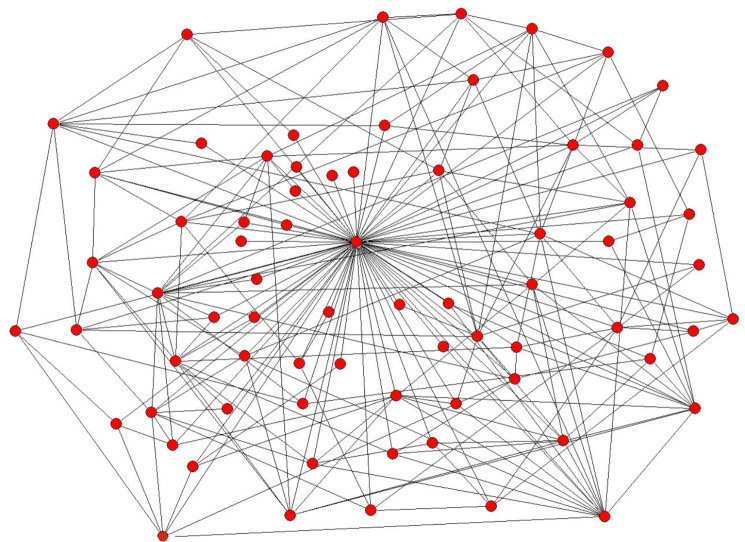
\includegraphics[scale=0.23]{graph}
\end{figure}
\end{center}
\end{frame}


\begin{frame}{The transition Matrix}
The transition matrix of our Markov Chain is:

$$
P = \alpha 1^T J + (1-\alpha) R
$$

where:
\begin{itemize}
\item $\alpha$ is the probability of moving to a random page.
\item $1^T$ is a unitary vector in the space of nodes.
\item $J$ is a constant vector in the space of nodes, that regulates the accessibility of nodes during the jumps.
\item $R$ is a matrix where $R_{i,j}$ is the probability of moving from node i to node j, i.e. $\frac{1}{\text{\# outgoing edges from i}}$ if $j$ is in the neighborhood of $i$, $0$ otherwise.
\end{itemize}

\end{frame}

\begin{frame}{The score vector}
\begin{block}{Theorem}
The score vector $\pi$ is the unique stochastic eigenvector of $P$ corresponding to the eigenvalue $1$:
$$
\pi P = \pi.
$$
\end{block}

Since the matrix $P$ has in practice thousands or millions of rows, solving exactly the system is not feasible and so we compute an approximation by using an iterative schema:

\begin{enumerate}
\item Let $\pi_0$ be our approximated solution.
\item Initialize $\pi_0$.
\item Set $\pi_{t+1}$ = $\pi_{t} P$ while $|\pi_{t+1} - \pi_t| \geq \epsilon$, where $\epsilon$ is a fixed tolerance.
\end{enumerate}

\end{frame}

\begin{frame}[fragile]{PageRank Implementation}

\begin{lstlisting}[basicstyle=\tiny]
def PageRank(R, alpha = .2, J = None, S: list = None, x_0 = None, eps = 10**(-2)):
    '''
    Implementation of the PageRank algorithm using an iterative
    method.
    
    Inputs:
    
    R:       stochastic transition matrix
    alpha:   damping factor
    J:       jump vector
    S:       list of pages specific to a certain topic
    x_0:     initial guest
    eps:     precision
    
    Outputs:
    
    pi:      PageRank vector
    error:   approximation error at every iteration
    it:      number of iterations to reach convergence
    '''
    
    # number of nodes
    tmp = R.shape[0]
    # initialize x_0
    if x_0 is None:
        x_0 = np.random.rand(1,tmp)
\end{lstlisting}

\end{frame}


\begin{frame}[fragile]{PageRank Implementation}

\begin{lstlisting}[basicstyle=\tiny]
	# initialize J/J_{S}
    if S is not None:
        # the number of pages specific to a certain topic
        # can not be greater than the overall number of
        # pages in the dataset  
        assert len(S) <= R.shape[0] 
        # if S is given than J must be None since it would be
        # automatically deduced from S
        assert J is None
        J = np.array([1/len(S) if i in S else 0 for i in range(tmp)])
    else:
        if J is None:
            # basic version of J with equal probabilities
            J = np.ones(shape=(1,tmp)) * (1/tmp)
    
    J = np.reshape(J, (1,tmp))
    # initialize x_{t+1}
    pi = x_0 + 1
    # initialize 1
    one_vector = np.ones(shape=(tmp,1))
    # initialize the error vector
    error = [np.linalg.norm( pi - x_0 )]
    # iterative matrix
    P = alpha * np.matmul(one_vector, J) + (1 - alpha) * R
    
    it = 1
    while np.linalg.norm( pi - x_0 ) >= eps:
        # do computations
        _ = np.matmul(x_0, P)
        # update
        x_0 = pi
        pi = _
        error.append(np.linalg.norm( pi - x_0))
        it += 1
        
    return pi.flatten(), error, it
    
\end{lstlisting}
\end{frame}

\begin{frame}{Weight Vector for the dataset}
The \href{www.cs.cornell.edu/courses/cs685/2002fa/data/gr0.California}{dataset} that I used to perform some experiments consists in a graph of 9664 websites and 16150 links. By performing the PageRank algorithm:
\begin{center}
\begin{figure}[h] 
\centering 
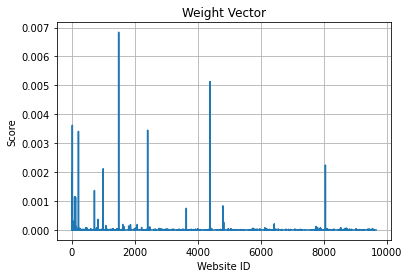
\includegraphics[scale=0.4]{pi}
\end{figure}
\end{center}
\begin{center}
\begin{figure}[h] 
\centering 
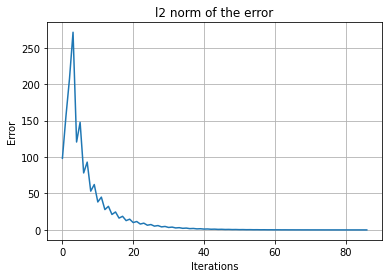
\includegraphics[scale=0.3]{error}
\end{figure}
\end{center}
\end{frame}

\begin{frame}{Top 10 Websites}
We can now have a look at the top scoring pages according to $\pi$:
\begin{center}
\begin{figure}[h] 
\centering 
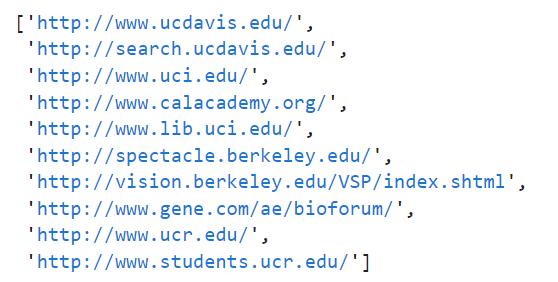
\includegraphics[scale=.8]{top10}
\end{figure}
\end{center}


\end{frame}

\begin{frame}{Topic Specific PageRank}
We can force the user to jump only within a finite set of web pages in what is known as Topic Specific PageRank.
\\
if S is a subset of the nodes, the new $J_S$ is defined as:
$$ (J_S)_{i} = 
\begin{cases}
  \frac{1}{|S|} & i \in S \\
       0 & \text{otherwise} 
\end{cases}
$$
And now solve the system with: $$P_S = \alpha 1^T J_S + (1-\alpha) R.$$
By setting S to the first 10 webpages:
\begin{figure}[!tbp]
  \centering
  \begin{minipage}[b]{0.4\textwidth}
    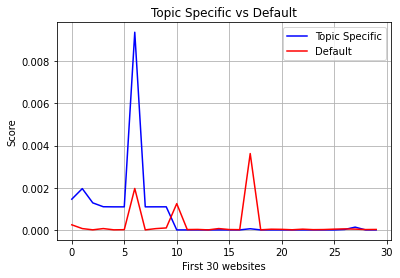
\includegraphics[width=\textwidth]{first30}
    %\caption{}
  \end{minipage}
  \hfill
  \begin{minipage}[b]{0.4\textwidth}
    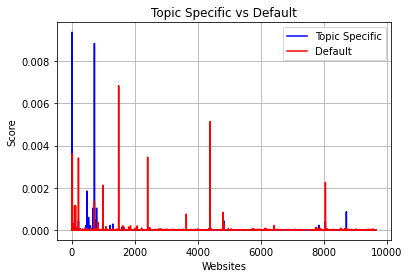
\includegraphics[width=\textwidth]{first30_2}
    %\caption{Flower two.}
  \end{minipage}
\end{figure}
\end{frame}

\begin{frame}{Topic Specific PageRank}
Let's now define S as a list of 100 randomly sampled website:
\begin{center}
\begin{figure}[h] 
\centering 
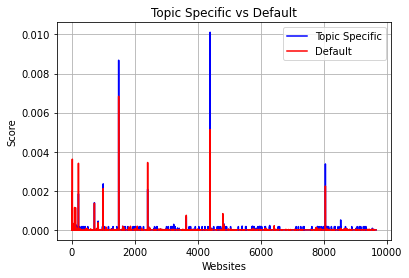
\includegraphics[scale=0.6]{random100}
\end{figure}
\end{center}

Since the Topic Specific websites were selected at random the final effect is basically that we averaged the scores all over the nodes, with just few very important websites

\end{frame}

\begin{frame}{Experiments on $\alpha$}
We modify the damping factor $\alpha$ and see how it affects the score vector:

\begin{figure}[!tbp]
  \centering
  \begin{minipage}[b]{0.4\textwidth}
    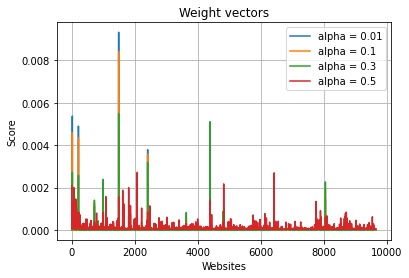
\includegraphics[width=\textwidth]{alpha1}
    %\caption{}
  \end{minipage}
  \hfill
  \begin{minipage}[b]{0.4\textwidth}
    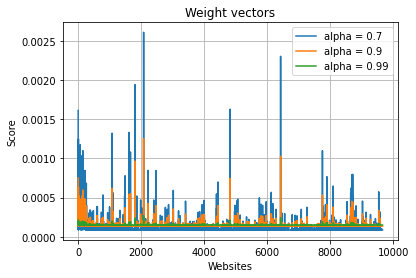
\includegraphics[width=\textwidth]{alpha2}
    %\caption{Flower two.}
  \end{minipage}
\end{figure}
We can conclude that the greater the value of alpha the more uniform the distribution of the weights is. A greater $\alpha$ means greater probability of randomly jumping from one node to another and so all the nodes tend to achieve similar importance.

\end{frame}

\begin{frame}{Impact of $\alpha$ on the number of iterations}
We modify the damping factor $\alpha$ and see how it affects the number of iterations needed to reach convergence:

\begin{center}
\begin{figure}[h] 
\centering 
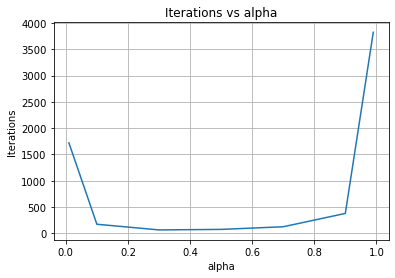
\includegraphics[scale=0.65]{it_vs_alpha}
\end{figure}
\end{center}
It looks like extreme values of $\alpha$ imply more iterations to reach convergence.

\end{frame}



 

\end{document}